\documentclass[scheme=chinese,a4paper]{report}
% \documentclass{report}
\usepackage[utf8]{inputenc}
\usepackage{amsmath}
\usepackage{esint}
\usepackage{tabstackengine}
\usepackage[colorlinks,linkcolor=blue]{hyperref}
\usepackage{xeCJK}
\usepackage{caption} 
\usepackage{stackengine}
\usepackage{graphicx}
\graphicspath{ {../resources/figure/digi/} }
\usepackage{float}
\usepackage{amsmath}
\usepackage{ulem}
\usepackage{amsfonts}

\usepackage{tikz}
\usetikzlibrary{calc}
\usepackage{pgfplots}
\usepackage{mathrsfs}
\usetikzlibrary{shapes,arrows}
\usetikzlibrary{arrows}
\captionsetup[table]{skip=10pt}

%%%% 下面的命令重定义页面边距,使其符合中文刊物习惯 %%%%
\addtolength{\topmargin}{-54pt}
\setlength{\oddsidemargin}{0.63cm}  % 3.17cm - 1 inch
\setlength{\evensidemargin}{\oddsidemargin}
\setlength{\textwidth}{14.66cm}
\setlength{\textheight}{24.00cm}    % 24.62

%%%% 段落首行缩进两个字 %%%%
% \makeatletter
% \let\@afterindentfalse\@afterindenttrue
% \@afterindenttrue
% \makeatother
% \setlength{\parindent}{2em}  %中文缩进两个汉字位

% 段首不缩进
\setlength{\parindent}{0pt}
%%%% 下面的命令设置行间距与段落间距 %%%%
\linespread{1.4}
% \setlength{\parskip}{1ex}
\setlength{\parskip}{0.5\baselineskip}

\def\rlwd{.5pt} \def\rlht{2.2ex} \def\rldp{.5ex}
\def\mydiv#1{~%
  \rule[-\rldp]{\rlwd}{\rlht}%
  \setbox0=\hbox{~#1}%
  \stackunder[\dimexpr\rldp-\rlwd]{~#1}{\rule{\wd0}{\rlwd}}%
}

\title{Digi Note}
\author{Crosstyan}
\date{Augest 2020}
\begin{document}
  \chapter{Basic}
  \section{N-base}
  \section{N-base to Decimal}
  $$\text{Decimal}=\sum_{i=-m}^{n-1} k_i\cdot N^i $$
  N为相应进制的base, $ k_i$为i-th的系数. 整数部分有n位, 小数部分有m位. 
  $$ (1101.011)_B=1\times 2^3+ 1\times 2^2+ 0\times 2^1+ 1\times 2^0+ 0\times 2^{-1}+ 1\times 2^{-2}+ 1\times 2^{-3} $$
  \section{Bin to Oct or Hex}
  Oct 取三位Bin. (若不足三位之倍数则在最高位和最低位补齐). 
  \begin{table}
    \centering
    \caption{Oct to Bin}
    \begin{tabular}{c c}
      \hline
      Bin&Oct\\
      \hline
      000&0 \\
      001&1 \\
      010&2 \\
      011&3 \\
      100&4 \\
      101&5 \\
      110&6 \\
      111&7 \\
    \end{tabular}
  \end{table}
  \begin{table}
    \centering
    \caption{Hex to Bin}
      \begin{tabular}{ll}
        \hline
        Hex&Bin\\
        \hline
      0     & 0000 \\
      1     & 0001 \\
      2     & 0010 \\
      3     & 0011 \\
      4     & 0100 \\
      5     & 0101 \\
      6     & 0110 \\
      7     & 0111 \\
      8     & 1000 \\
      9     & 1001 \\
      A     & 1010 \\
      B     & 1011 \\
      C     & 1100 \\
      D     & 1101 \\
      E     & 1110 \\
      F     & 1111 \\
      \end{tabular}%
  \end{table}%
  $$ (3D.BE)_{H}= \underset{3}{0011} \, \underset{D}{1101} \,.\, \underset{B}{1011}\, \underset{E}{1110}=(11\,1101.1011\,111)_B$$
  Hex取四位Bin. (若不足四位之倍数则在最高位和最低位补齐). 
  $$ (1001.1101)_B=001\,001.110\,100=\underset{1}{001}\,\underset{1}{001}\,.\,\underset{6}{110}\,\underset{4}{100}=(11.64)_O $$
\section{Dec to n-base}
\subsection{整数}
短除法, 除到余数为零. \\
\begin{tabular}{rl} 
2\mydiv{25} &\\
2\mydiv{12}  & remainder 1\\
2\mydiv{6}  & remainder 0\\
2\mydiv{3}   & remainder 0\\
2\mydiv{1}            & remainder 1\\
0&remainder 1
\end{tabular}

得到的数字, 下方为高位, 上方为低位. (最后一次运算为最高位) 即结果为$(1\,1001)_B$
\subsection{小数}
加倍取整数为当前位, 然后取其小数作为下一位之运算. 
\begin{align}
    0.125\times 2 = \underset{0}{0.}25 \\
    0.25\times 2 = \underset{0}{0.}5\\
    0.5\times 2=\underset{1}{1.}0
\end{align}
即小数部分为$0.001$ (最后一次运算为最低位)
\section{compliment}
\subsection{1's compliment (反码)}
按位取反, 最高位保留一个符号位. (0为正, 1为负)
\subsection{2's compliment (补码)}
负数的情况下, 1's compliment 加 $ (0001)_B $ 即可 (正数不变)
\section{Encoding}
\subsection{BCD Code}
\subsubsection{8421 BCD}
8421就是按照十进制拆数, 每位数用对应的二进制码表示+\par

\begin{table}[htb]
    \centering
    \caption{Dec to 8421}
    \begin{tabular}{c c}
        Dec & 8421 \\
        \hline
        10 & 0001 0000\\
        11 & 0001 0001\\
        12 & 0001 0010\\
        20 & 0010 0010\\
        21 & 0010 0001\\
    \end{tabular}
\end{table}
0至9与Binary相同. 

\subsubsection{Excess-3 (XS-3)}
就是8421每一位加三. 
\begin{itemize}
    \item Find the decimal equivalent of the given binary number.
    \item Add +3 to each digit of decimal number.
    \item Convert the newly obtained decimal number back to binary number to get required excess-3 equivalent.
\end{itemize}

% Table generated by Excel2LaTeX from sheet 'Sheet1'
\begin{table}[htb]
    \centering
    \caption{Dec, 8421 and Excess-3}
      \begin{tabular}{c c c}
        Dec& 8421 & Excess-3\\
        \hline
      0     & 000     & 011 \\

      1     & 001     & 100 \\

      2     & 010    & 101 \\

      3     & 011    & 110 \\

      4     & 100   & 111 \\

      5     & 101   & 1000 \\

      6     & 110   & 1001 \\

      7     & 111   & 1010 \\

      8     & 1000  & 1011 \\

      9     & 1001  & 1100 \\
      \end{tabular}%
  \end{table}%
  

\subsubsection{Grey Code}
% Table generated by Excel2LaTeX from sheet 'Sheet1'
\begin{table}[htb]
    \centering
    \caption{Bin to Gray}
      \begin{tabular}{rl}
      \multicolumn{1}{l}
      {Bin} & Gray \\
      \hline
      000     & 000 \\
      001     & 001 \\
      010     & 011 \\
      011     & 010 \\
      100     & 110 \\
      101     & 111 \\
      110     & 101 \\
      111     & 100 \\
      \end{tabular}%
    \label{tab:addlabel}%
  \end{table}%
  
$$ G(n)=B(n+1) \, XOR \, B(n) $$
$$ G(n) = B(n+1) + B(n) $$
自低位至高位运算即可,无需考虑进位. 
$$ B(n) = -B(n+1)+ G(n) $$
自高位至低位运算即可,无需考虑借位. 


\chapter{Boolean Algebra}
\section{Operator}
\subsection{AND}
$$A\cdot B$$
\begin{table}[htb]
    \centering
    \begin{tabular}{c c c}
    A&B&$A\cdot B$\\
    \hline
    0&0&0\\
    0&1&0\\
    1&0&0\\
    1&1&1\\
    \end{tabular}
    \caption{AND Truth Table}
\end{table}

\subsection{OR}
$$A+B$$
\begin{table}[htb]
    \centering
    \begin{tabular}{c c c}
    A&B&A+B\\
    \hline
    0&0&0\\
    0&1&1\\
    1&0&1\\
    1&1&1\\
    \end{tabular}
    \caption{OR Truth Table}
\end{table}

\subsection{Exclusive OR/XOR}
\begin{table}[htb]
    \centering
    \begin{tabular}{c c c}
    A&B&$A\oplus B$\\
    \hline
    0&0&0\\
    0&1&1\\
    1&0&1\\
    1&1&0\\
    \end{tabular}
    \caption{XOR Truth Table}
\end{table}

From the truth table we can get that. 
$$A \oplus B=A^\prime B+AB^\prime$$

\subsection{Exclusive NOR/XNOR}
\begin{table}[htb]
    \centering
    \begin{tabular}{c c c}
    A&B&$A\odot B$\\
    \hline
    0&0&1\\
    0&1&0\\
    1&0&0\\
    1&1&1\\
    \end{tabular}
    \caption{XNOR Truth Table}
\end{table}

From the truth table we can get that. 
$$A \odot B=A^\prime B^\prime+AB$$

\subsection{NOT}
$$A^\prime$$
\subsection{与或非}
俩与门加一或非门(two AND then a NOR)
四个输入变量
\section{Formula}
\subsection{代数公理}
A和0, A和1
\begin{align*}
    A\cdot 0=0\\
    A\cdot 1=A\\
    A+0=A\\
    A+1=1
\end{align*}
A和A, A和NOT A
\begin{align*}
A\cdot A=A\\
A +A=A\\
A\cdot A^\prime=0\\
A+A^\prime=1
\end{align*}
\subsection{等同律}
\begin{align*}
    A+A^\prime\cdot B &= A\cdot 1+A^\prime\cdot B\\
    &=A\cdot(1+B)+A^\prime\cdot B\\
    &=A+AB+A^\prime B\\
    &=A+(A^\prime+A)\cdot B\\
    &=A+B
\end{align*}
\subsection{吸收律}
\begin{align*}
    A(A+B) &= A+AB\\
    &=A\cdot(1+B) && \text{ONE OR anything is always ONE}\\ 
    &=A
\end{align*}

\subsection{De Morgan's law}
$$(AB)^\prime=A^\prime+B^\prime$$
$$(A+B)^\prime=A^\prime\cdot B^\prime$$
\subsection{分配律}
\begin{align}
    A+B\cdot C=(A+B)\cdot (A+C) && \text{AND distributive law}\\
    A\cdot (B+C)=AB+AC && \text{OR distributive law}
\end{align}
\subsection{A something OR NOT A something else}
(A AND $Other_1$) OR (NOT A AND $Other_2$) OR ($Other_1$ AND $Other_2$ AND $Other_3$...)\par
\begin{align*}
    AB+A^\prime C+BC=AB+A^\prime C &&\text{舍去最后一项} \\
    AB+A^\prime C+BCD=AB+A^\prime C\\
    AB+A^\prime C+BCDE=AB+A^\prime C &&\text{不管有多少项相乘}
\end{align*}
两个乘积项分别包含 $ A $和 $ A ^\prime$两个因子, 其余因子正好组成第三个乘积项或其一部分, 这一项则可以被消去. 
\subsection{对偶性(Duality)}
如果两个逻辑式子相等, 则他们的对偶式亦相等\\
求Duality, 就是把OR变AND, 把AND变OR.(注意和求反区别)
\begin{align*}
    A+B\cdot C &=(A+B)\cdot (A+C) && \text{AND distributive law}\\
    (A+B\cdot C)^D &=[(A+B)\cdot (A+C)]^D\\
    A\cdot (B+C) &=AB+AC && \text{OR distributive law}
\end{align*}
\section{Truth Table to Boolean Expression}
右边取1的组合写下来做SOP即可. 
\section{逻辑表达式化为标准形式}
\subsection{最小项}
即SOP\\
写K-map, (四变量时左边为前俩, 上边为后俩), (三变量时左边为第一, 上边为后俩).
(标最小项时还是一行一行过去的)
然后按照二进制顺序排列即可得到最小项. \\
\sout{说白了最小项就是按照二进制顺序排列.} 更准确地说, 最小项就是把二进制转换成对应的十进制. 
\paragraph{例子} $AB'CD'EF$按照原变量为1, 反变量为0可以得到$(101011)_B$转换为十进制数为$(43)_D$则其编号就是$43$. $AB'CD'EF$有6个变量, 即一共有$2^6=64$项
\subsection{最大项}
即POS. \\
最小项于最大项为互补关系. 即$m_i^\prime=M_i$, $M_i^\prime=m_i$\\
列个真值表或者画个卡诺图, 已知最小项(为1的), 剩下的(为0的)就是最大项了\\
$$Y=\sum_{i} m_i=\prod_{k\neq i} M_k$$
\section{K-map}
写K-map, (四变量时左边为前俩, 上边为后俩), (三变量时左边为第一, 上边为后俩).\\
别忘了四角是可以互通的 (或者上边俩角, 或者下边俩角, 但是对角线是不能互通的). 
\section{SOP and POS}
\subsection{SOP和NAND}
\subsection{POS和NOR}

\chapter{CMOS门电路}
FET P channel\footnote{NPN is not pointing in} is pointing out. \\
P沟道指出去
\section{CMOS NOT}
\begin{figure}[H]
    \centering
    \includegraphics[width=0.33\textwidth]{cmos_not.png}
    \caption{CMOS NOT}
\end{figure}
T channel Serializing N channel is NOT Gate.\\T串N
\section{CMOS NAND}
\begin{figure}[H]
\centering
\includegraphics[width=0.33\textwidth]{cmos_nand.png}
\caption{CMOS NAND}
\end{figure}
T channels Serializing, P channels Paralleling together are NAND gate. \\
T相串P相并为NAND
\section{CMOS NOR}
\begin{figure}[H]
    \centering
    \includegraphics[width=0.33\textwidth]{cmos_nor.png}
    \caption{CMOS NOR}
    \end{figure}
T channels Paralleling, P channels Serializing together are NOR gate. \\
P相串T相并为NOR
\section{OD Gate}
\begin{figure}[H]
\centering
\includegraphics[width=0.33\textwidth]{cmos_od.png}
\caption{OD Gate}
\end{figure}
漏极开路门, 必须有个上拉电阻. 
\section{Transmission Gate}
\begin{figure}[H]
\centering
\includegraphics[width=0.33\textwidth]{cmos_tranmission.png}
\caption{Transmission}
\end{figure}
传输门, 就一电子开关. \par
上下分别为NOT C和C, 若下边的C为1(上边NOT C为0)则左右导通, 反之截止. 
\section{三态门}
\begin{figure}[H]
\centering
\includegraphics[width=0.33\textwidth]{cmos_tri_condition.png}
\caption{三态门}
\end{figure}
其有三种状态: 高电平, 低电平, 高阻态\par
就一非门, 只不过多了一个高阻态. \par
当$EN^\prime=0$时为正常非门(低电平有效, 有效就是作为非门正常工作)\par
$EN^\prime=1$为高阻态.
\section{噪声容限}
\begin{align*}
    V_{NH}=V_{(\text{OH min})}-V_{(\text{IH min})}\\
    V_{NL}=V_{(\text{IL max})}-V_{(\text{OL max})}
\end{align*} 

\begin{figure}[H]
\centering
\begin{tikzpicture}
\coordinate (rec_st) at (0,0);
\coordinate (rec_e) at (1,6);
\coordinate (dist) at (4,0);
\coordinate (rec2_st) at ($(rec_st)+(dist)$);
\coordinate (rec2_e) at ($(rec_e)+(dist)$);
\coordinate (OH) at (0,5.5);
\coordinate (OL) at (0,.5);
\coordinate (IH) at ($(rec2_st)+(0,4.5)$);
\coordinate (IL) at ($(rec2_st)+(0,1.5)$);

\draw (rec_st) rectangle (rec_e);
\draw (rec2_st) rectangle (rec2_e);

\draw (IH) node[below left]{$V_{\text{IH (min)}}$}--+(1,0)--+(-1.5,0) node(IH_e)[]{};
\draw (IL) node[above left]{$V_{\text{IL (max)}}$}--+(1,0)--+(-1.5,0) node(IL_e)[]{};


\draw (OH)--++(1,0) node[above right]{$V_{\text{OH (min)}}$}--+(1.5,0)  node(OH_e)[]{};
\draw (OL)--++(1,0) node[below right]{$V_{\text{OL (max)}}$}--+(1.5,0)  node(OL_e)[]{};

\draw[<->] (IL_e)--node[right]{$V_{\text{NL}}$}(OL_e);
\draw[<->] (OH_e)--node[right]{$V_{\text{NH}}$}(IH_e);

\node [] at ($(rec_st)!0.5!(rec_e)$) {$v_\text{out}$} ;
\node [] at ($(rec2_st)!0.5!(rec2_e)$) {$v_\text{in}$} ;

\draw [->] ($(rec_st)+(-1,0)$)--(-1,7) node[right]{$v$};
\end{tikzpicture}
\caption{噪声容限}
\end{figure}
\section{CMOS门注意事项}
\begin{itemize}
    \item 不允许出现悬空端
    \item NAND接1 ($1\cdot A=A$)
    \item NOR接0 ($0+A=A$)
    \item TTL可悬空, 若悬空则为高电平
\end{itemize}
\chapter{组合逻辑电路}
\begin{itemize}
    \item 逻辑抽象
    \item 真值表
    \item 写出表达式
    \item 化简表达式
    \item 画出门电路图
\end{itemize}
\section{常用模型}
\subsection{Full Adder}
被加数, 加数, Carry in, Sum, Carry out. \par
半加器不包含Carry in. 
% Table generated by Excel2LaTeX from sheet 'Sheet1'
\begin{table}[htb]
    \centering
    \caption{Truth table of Full Adder}
      \begin{tabular}{rrr|rr}
      \multicolumn{1}{l}{A} & \multicolumn{1}{l}{B} & \multicolumn{1}{l}{$ C_{in} $} & \multicolumn{1}{l}{Sum} & \multicolumn{1}{l}{$ C_{out} $} \\
      0     & 0     & 0     & 0     & 0 \\
      0     & 0     & 1     & 1     & 0 \\
      0     & 1     & 0     & 1     & 0 \\
      0     & 1     & 1     & 0     & 1 \\
      1     & 0     & 0     & 1     & 0 \\
      1     & 0     & 1     & 0     & 1 \\
      1     & 1     & 0     & 0     & 1 \\
      1     & 1     & 1     & 1     & 1 \\
      \end{tabular}%
    \label{tab:addlabel}%
  \end{table}%
  
\subsection{Full Subtractor}
被减数, 减数, Borrow in, Difference, Borrow out. \par
半减器不包含Borrow in. 
% Table generated by Excel2LaTeX from sheet 'Sheet1'
\begin{table}[htb]
    \centering
    \caption{Truth table of Full Subtractor}
      \begin{tabular}{rrr|rr}
      \multicolumn{1}{l}{Minuend} & \multicolumn{1}{l}{Subtrahend} & \multicolumn{1}{l}{$ B_{in} $} & \multicolumn{1}{l}{Diff} & \multicolumn{1}{l}{$ B_{out} $} \\
      0     & 0     & 0     & 0     & 0 \\
      0     & 0     & 1     & 1     & 1 \\
      0     & 1     & 0     & 1     & 1 \\
      0     & 1     & 1     & 0     & 1 \\
      1     & 0     & 0     & 1     & 0 \\
      1     & 0     & 1     & 0     & 0 \\
      1     & 1     & 0     & 0     & 0 \\
      1     & 1     & 1     & 1     & 1 \\
      \end{tabular}%
    \label{tab:addlabel}%
  \end{table}%
\section{竞争冒险(race hazard)}
\subsection{Race}
两个输入端信号同时向相反方向变化, 变化的时间有差异时为Race. 
\subsection{Hazard}
两个输入端变化方向相反时, 由Race产生的可能出现的. 由于\textbf{电路中出现延时而引起的}. \par
当一个门电路的输入公式在某些情况下可以化为两个互补信号的AND ($ A\cdot A ^\prime $) 或OR ($ A+A ^\prime $) 时就有可能出现race hazard. 
\subsubsection{消除方法}
\begin{itemize}
    \item 接入滤波电容
    \item 引入选通脉冲
    \item 增加冗余项, 使得最终结果不可能出现两个互补信号. 
\end{itemize}
\subsubsection{增加冗余项}
\label{eg:hazard}
$$ Y=AB+A ^\prime C $$ 当 $ B=C=1 $时, $ Y=A+A ^\prime $. 
若增加一个冗余项, 变为 $$ Y=AB+A ^\prime C+BC $$
当 $ B=C=1 $时, $ Y=A+A ^\prime+1=1 $. 避免了最终结果的两个互补变量的出现. 
\chapter{集成逻辑电路}
\section{Encoder}
好像不考\\
所谓编码器(74LS148)\\
注意输入是高电平有效还是低电平有效, 注意输出是输出原变量还是反变量. \\
$2^n$个输入端口, $n$个输出端口. 将输入的输入端口序号用二进制进行编码. (同时只能有一个有效输入)
\begin{figure}[H]
    \centering
    \includegraphics[width=0.33\textwidth]{Encoder_block_diagram.jpg}
    \caption{encoder}
\end{figure}


% Table generated by Excel2LaTeX from sheet 'Sheet1'
\begin{table}[H]
    \centering
    \caption{Truth Table of 8 to 3 Encoder}
      \begin{tabular}{cccccccc|ccc}
      \multicolumn{8}{c}{INPUT}                                     & \multicolumn{3}{c}{OUTPUT} \\
      $I_7$  & $I_6$  & $I_5$  & $I_4$  & $I_3$  & $I_2$  & $I_1$  & $I_0$  & $O_2$  & $O_1$  & $O_2$ \\
      0     & 0     & 0     & 0     & 0     & 0     & 0     & 0     & X     & X     & X \\
      0     & 0     & 0     & 0     & 0     & 0     & 0     & 1     & 0     & 0     & 0 \\
      0     & 0     & 0     & 0     & 0     & 0     & 1     & 0     & 0     & 0     & 1 \\
      0     & 0     & 0     & 0     & 0     & 1     & 0     & 0     & 0     & 1     & 0 \\
      0     & 0     & 0     & 0     & 1     & 0     & 0     & 0     & 0     & 1     & 1 \\
      0     & 0     & 0     & 1     & 0     & 0     & 0     & 0     & 1     & 0     & 0 \\
      0     & 0     & 1     & 0     & 0     & 0     & 0     & 0     & 1     & 0     & 1 \\
      0     & 1     & 0     & 0     & 0     & 0     & 0     & 0     & 1     & 1     & 0 \\
      1     & 0     & 0     & 0     & 0     & 0     & 0     & 0     & 1     & 1     & 1 \\
      \end{tabular}%
  \end{table}%
  \subsection{优先译码器}
  正常来说只能同时有一个输入, 输入为对应的输入端口序号的二进制编码. \\
  优先编码器可以同时运行多个输入, 按照$I_7>I_6>I_5>I_4>I_3>I_2>I_1>I_0$的优先级来决定输入, 即输入端口序号大者优先被输出. 

\section{Decoder}
所谓译码器(74LS138)\\
$n$个输入, $2^n$个输出. 注意看输出为低电平还是高电平. 
\begin{figure}[H]
    \centering
    \includegraphics[width=0.33\textwidth]{decoder-block-diagram.jpg}
    \caption{3 to 8 decoder}
\end{figure} 
% Table generated by Excel2LaTeX from sheet 'Sheet1'
\begin{table}[H]
    \centering
    \caption{Truth Table of 2 to 4 decoder}
      \begin{tabular}{c|cc|cccc}
      Enable & \multicolumn{2}{c}{Inputs} & \multicolumn{4}{c}{Outputs} \\
      E     & $A_1$    & $A_0$    & $Y_3$    & $Y_2$    & $Y_1$    & $Y_0$ \\
      0     & $x$     & $x$     & 0     & 0     & 0     & 0 \\
      1     & 0     & 0     & 0     & 0     & 0     & 1 \\
      1     & 0     & 1     & 0     & 0     & 1     & 0 \\
      1     & 1     & 0     & 0     & 1     & 0     & 0 \\
      1     & 1     & 1     & 1     & 0     & 0     & 0 \\
      \end{tabular}%
  \end{table}%
\subsection{利用Decoder和NAND门来表示SOP}
一个SOP表达式可以用Decoder\footnote{这里的Decoder输出为反变量, 若输出原变量则是用OR门}和NAND门来表示. \\

\begin{figure}[H]
\centering
\includegraphics[width=0.5\textwidth]{decoder.png}
\caption{Decoder与NAND表示SOP}
\end{figure}
上图表示$Z=A'B'C+A'BC'+AB'C'+ABC$, 化为最小项为$Z=m_1+m_2+m_4+m_7$. 
\section{Multiplexer}
可以理解为是一个decoder用作电子开关. 有$2^n$个输入和$1$个输出, $n$个控制端. 
\begin{figure}[H]
\centering
\includegraphics[width=0.5	\textwidth]{1920px-Multiplexer_8-to-1.svg.png}
\caption{ 3:8 MUX }
\end{figure}
% Table generated by Excel2LaTeX from sheet 'Sheet1'
\begin{table}[H]
    \centering
    \caption{Truth table of 2:4 MUX}
      \begin{tabular}{cc|c}
      \multicolumn{2}{c}{Selection Lines} & Output \\
      $S_1$    & $S_0$    & Z \\
      0     & 0     & $I_0$ \\
      0     & 1     & $I_1$ \\
      1     & 0     & $I_2$ \\
      1     & 1     & $I_3$ \\
      \end{tabular}%
  \end{table}%
$$Z=S_1'\cdot S_0'\cdot I_0+S_1'\cdot S_0\cdot I_1+S_1\cdot S_0'\cdot I_2+S_1\cdot S_0\cdot I_3$$
\subsection{MUX与三变量表达式}
三变量的话列出真值表就好了, 然后将真值表的输出填入到输入端口. 
\paragraph{例子} 用MUX实现$F=A\oplus B\oplus C$. \\
\label{eg:mux_1}
先列出真值表
% Table generated by Excel2LaTeX from sheet 'Sheet1'
\begin{table}[H]
    \centering
    \caption{$F=A\oplus B\oplus C$的真值表}
      \begin{tabular}{ccc|c}
      A     & B     & C     & F \\
      \hline
      0     & 0     & 0     & 0 \\
      0     & 0     & 1     & 1 \\
      0     & 1     & 0     & 1 \\
      0     & 1     & 1     & 0 \\
      1     & 0     & 0     & 1 \\
      1     & 0     & 1     & 0 \\
      1     & 1     & 0     & 0 \\
      1     & 1     & 1     & 1 \\
      \end{tabular}%
  \end{table}%
换句话说, 用SOP表示, 将SOP有的项转换成\textbf{最小项所对应的端口}的值为1. 
\begin{figure}[H]
\centering
\includegraphics[width=0.5\textwidth]{mux_1.png}
\caption{MUX与三变量表达式}
\end{figure}

\subsection{MUX与四变量表达式}
从外面额外引入第四个变量. SOP中的P可以被拆成$A\cdot BCD$之类的玩意\sout{ (就肯定又一个变量是做控制端的).} \\
这么描述也不太对\dots 反正肯定有第四个变量是从外面引入的. 
\begin{figure}[H]
    \centering
    \includegraphics[width=.5\textwidth]{mux_2.png}
    \caption{四变量表达式的MUX的例子}
    \end{figure}
    $ABC$决定输入的端口, 而$D$决定输入的端口的信号内容. 
\begin{itemize}
    \item $\mathbb{D}_0$接地为0. SOP表达式肯定没$A'B'C'$这项
    \item $\mathbb{D}_1,\mathbb{D}_5$和$D$相连. 即$A'B'C\cdot D,AB'C\cdot D$
    \item $\mathbb{D}_4,\mathbb{D}_6$和$D'$相连. 即$AB'C'\cdot D',ABC'\cdot D'$
    \item $\mathbb{D}_2,\mathbb{D}_7$恒为1. 即$A'BC',ABC$
\end{itemize}
最后结果为
$$Y=A'B'C\cdot D+AB'C\cdot D+AB'C'\cdot D'+ABC'\cdot D'+A'BC'+ABC$$


\subsection{数据选择器}
就是MUX的别称, 没什么特别的. 
\section{Demultiplexer}
不考
\subsection{数据分配器}
Demux别称. 

\chapter{Latch and Flip Flop}
\section{锁存器(Latch)}
Latch不怎么考, 就是没有CLK的FF, 一遇到输入信号就改变状态. 
\subsection{SR Latch}
\begin{figure}[H]
\centering
\includegraphics[width=0.5\textwidth]{rs_latch.png}
\caption{SR Latch}
\end{figure}


\section{Flip Flop}
有CLK的Latch. \\
FF的输出状态取决于输入信号和电路的原始状态. \\
FF的CP端如果有$\triangleright$则表示rising edge (上升沿), 若在前面加一个$\circ$表示NOT的话则为falling edge (下降沿)
\subsection{D FF}

\begin{figure}[H]
\centering
\includegraphics[width=0.5\textwidth]{d_ff.png}
\caption{D FF}
\end{figure}
$$ Q_\text{next}=D $$
\subsection{SR FF}
S for set (set to 0), R for reset (set to 1). \\
注意看输入是高电平有效还是低电平有效. 
% Table generated by Excel2LaTeX from sheet 'Sheet1'
\begin{table}[htb]
    \centering
    \caption{Truth Table of SR FF}
      \begin{tabular}{cc|c}
      \multicolumn{1}{l}{$S$} & \multicolumn{1}{l}{$R$} & $Q_\text{next}$ \\
      \hline
      0     & 0     & $Q$ \\
      0     & 1     & 0\\
      1     & 0     & 1\\
      1     & 1     & unknown \\
      \end{tabular}%
  \end{table}%
  
$$
\begin{cases}
    Q_\text{next}=S+R ^\prime\cdot Q\\
    S\cdot R=0 \qquad \text{(S与R不能同时取1)}
\end{cases}
$$

\subsection{JK FF}
\begin{figure}[H]
\centering
\includegraphics[width=0.33\textwidth]{jk_ff.png}
\caption{JK FF}
\end{figure}

\begin{table}[htb]
    \centering
    \caption{Truth Table of JK FF}
      \begin{tabular}{cc|c}
      \multicolumn{1}{l}{J} & \multicolumn{1}{l}{K} & $Q_\text{next}$ \\
      \hline
      0     & 0     & Q \\
      0     & 1     & 0\\
      1     & 0     & 1\\
      1     & 1     & $Q ^\prime$ \\
      \end{tabular}%
  \end{table}%
$$Q_\text{next}=J\cdot Q ^\prime+K ^\prime\cdot Q$$
J相当于Set, K相当于Reset. 
\subsection{JK触发器转换}
若$J=K(=T)$,可完成$T$ FF的逻辑功能, $J=K'(=D)$可以完成$D$ FF的逻辑功能
\subsection{T FF}
T for toggle. 
\begin{figure}[H]
\centering
\includegraphics[width=0.33\textwidth]{t_ff.png}
\caption{T FF}
\end{figure}
$$Q_\text{next}=T\cdot Q ^\prime+ T ^\prime \cdot Q$$
\begin{table}
    \centering
    \caption{Truth Table for T FF}
    \begin{tabular}{c|c}
        T&$Q_\text{next}$\\
        \hline
        0&Q\\
        1&$Q ^\prime$\\
    \end{tabular}
\end{table}
\subsection{触发方式}
\subsubsection{主从触发}
\subsubsection{边缘触发}
\subsection{带异步置位/复位的FF}
当异步复位端有效时, 输出$Q$被强制转换为0. \\
置位端则使得$Q$被强制转换为1. \\
由于是异步, 所以无视时钟$CLK$直接输出直接变化. 
\section{FF之间的转换}
\begin{itemize}
    \item 写出两种FF的特性方程
    \item 对比转换电路的表达式
    \item 用门电路和目标FF画出转换电路
\end{itemize}
\subsection{D FF to JK FF}
\sout{ \text{Realise $J(D)$和$K(D)$}  (目标FF的输入变量为当前FF的输入变量的函数)} 只需要找到它们之间的关系即可, 不一定谁是谁的函数. 
\begin{align*}
    Q_\text{next}=D=D\cdot (Q+Q ^\prime)&=D\cdot Q+ D \cdot Q ^\prime \\
    Q_\text{next}&=J\cdot Q ^\prime+ K ^\prime \cdot Q &&\text{RHS 相等}\\
    \begin{cases}
        J(D)=D\\
        K(D)=D ^\prime \qquad  \text{because }K ^\prime=D
    \end{cases}
\end{align*}

\subsection{JK FF to T FF}
\sout{目标: $T(J,K)$}
\begin{align*}
    Q_\text{next}&=J\cdot Q ^\prime+ K ^\prime \cdot Q \\
    Q_\text{next}&=T\cdot Q ^\prime+ T ^\prime \cdot Q \\
\end{align*}
$$
\begin{cases}
    J(T)=T\\
    K(T)=T ^\prime
\end{cases}
$$
\subsection{D FF to T FF}
\begin{align*}
    \begin{cases}
        Q_\text{next}&=D\\
        Q_\text{next}&=T\cdot Q ^\prime+ T ^\prime \cdot Q \\
    \end{cases}\\
    D(T,Q)=T\cdot Q ^\prime+ T ^\prime \cdot Q=T\oplus Q
\end{align*}
\chapter{时序逻辑电路分析}
\section{设计理论}
由组合逻辑电路和存储电路构成, 又被称作状态机. \par
\begin{itemize}
    \item Mealy 米利型 (输出和输入变量有关)
    \item Moore 摩尔型 (输出和输入变量无关)
\end{itemize}
描述方式:
\begin{itemize}
    \item 驱动方程 (FF的输入表达式/输入变量) (不包括CLK)
    \item 状态方程 (将驱动方程代入到FF的特性方程得到)
    \item 输出方程 (就是输出变量的表达式)
    \item 状态真值表(输入|现态|次态|输出)\footnote{有时候没有输入或者输出可不填写}
    \item 状态转换表 (次态/现态的输出)\footnote{Mealy型电路} (时钟|现态|输出)\footnote{异步}
    \item 状态转换图
\end{itemize}
将输入变量以及出台带入状态方程和输出方程, 求得次态和初态的输出, 将其作为新的初态循环. 结束之后需要检查是否包含所有的结果. 

\section{同步}

\subsection{Moore型}
\paragraph{例题}分析图中的电路, 描述其功能. \footnote{左下角空着的是时钟CLK, 右上角是输出$Z$}\\
摩尔型电路输出方程与输入无关. 
\begin{figure}[H]
\centering
\includegraphics[width=0.7\textwidth]{sync_example.png}
\caption{摩尔型电路例题}
\label{eg:sync_1}
\end{figure}
$\triangleright$前边有$\circ$故为falling edge. 
\subparagraph{驱动方程} 就是JK FF的输入. 
\begin{align*}
    \begin{cases}
        J_1=X\\
        K_1=X'
    \end{cases}
    \begin{cases}
        J_2=Q_1\\
        K_2=Q_1'
    \end{cases}
\end{align*}
\subparagraph{输出方程}右上角的AND gate大概就是输出. 
$$Z=Q_1\cdot Q_2'$$

\subparagraph{状态方程}将驱动方程JK FF的特征方程代入$Q^\star=J\cdot Q'+K'\cdot Q$可以得到
\begin{align*}
    Q^*_1&=X\cdot Q_1'+(X')'\cdot Q_1\\
    &=X\cdot Q_1'+X\cdot Q_1\\
    &=X\cdot(Q_1'+Q_1)\\
    &=X\\
    Q^*_2&=Q_1\cdot Q_2'+Q_1\cdot Q_2\\
    &=Q_1\cdot(Q_2'+Q_2)\\
    &=Q_1
\end{align*}

\subparagraph{状态转换表}
\sout{状态转换表又被称作状态转移真值表}如果是摩尔型\footnote{输出和输入变量无关}的电路则两者相同. 真值表顾名思义就是按照真值表二进制排列顺序列出来的东西 (区分那么多干啥, 两者似乎差不多)\\
得先假定一个输入, 在此我们先假设输入$X=0$\\
还得假设一个初态, 在此假设$Q_1,Q_2=0$\\
在此直接按照二进制顺序排列. 
% Table generated by Excel2LaTeX from sheet 'Sheet1'
\begin{table}[htbp]
    \centering
    \caption{状态转换表/状态真值表}
      \begin{tabular}{c|cc|cc|c}
      $X$     & $Q_1$    & $Q_2$    & $Q_1^*$   & $Q_2^*$   & $Z$ \\
      \hline
      0     & 0     & 0     & 0     & 0     & 0 \\
      0     & 0     & 1     & 0     & 0     & 0 \\
      0     & 1     & 0     & 0     & 1     & 1 \\
      0     & 1     & 1     & 0     & 1     & 0 \\
      1     & 0     & 0     & 1     & 0     & 0 \\
      1     & 1     & 0     & 1     & 1     & 1 \\
      1     & 1     & 1     & 1     & 1     & 0 \\
      1     & 0     & 1     & 1     & 0     & 0 \\
      \end{tabular}%
  \end{table}%
\subparagraph{状态转换图}如下图. (状态/输出) 为一个节点, 箭头指向次态, 箭头上方为输入. 
\begin{figure}[H]
\centering
\includegraphics[width=0.5\textwidth]{sync_example_graph.png}
\caption{状态转换图}
\end{figure}
\subsection{Mealy型}
\label{eg:sync_2}
米利型电路输出方程与输入无关. 
\paragraph{例题} 分析下列电路
\begin{figure}[H]
\centering
\includegraphics[width=0.7\textwidth]{sync_example_2.png}
\caption{米利型例题}
\end{figure}
\subparagraph{驱动方程}
\begin{align*}
    \begin{cases}
        J_1=1\\
        K_1=1
    \end{cases}
    \begin{cases}
        J_2=Q_1\oplus A\\
        K_2=Q_1\oplus A
    \end{cases}
\end{align*}
\subparagraph{输出方程}
\begin{align*}
    Y&=[(AQ_1 Q_2)'\cdot (A'Q_1'Q_2')']'\\
    &=AQ_1 Q_2+A'Q_1' Q_2'
\end{align*}
\subparagraph{状态方程}
\begin{align*}
    Q^*_1&=J_1\cdot Q_1'+K'\cdot Q_1\\
    &=Q_1'\\
    Q^*_2&=(Q_1\oplus A)\cdot Q_2'+(Q_1\oplus A)'\cdot Q_2\\
    &=(Q_1\oplus A)\cdot Q_2'+(Q_1\odot A)\cdot Q_2
\end{align*}
XOR取反为XNOR

\begin{align*}
    A\oplus B&=A'B+AB'\\
    (A\oplus B)'=A\odot B&= AB+A'B' 
\end{align*}
\subparagraph{状态真值表} (输入|现态|次态|输出) 如下表
% Table generated by Excel2LaTeX from sheet 'Sheet1'
\begin{table}[H]
    \centering
    \caption{状态真值表} 
      \begin{tabular}{c|cc|cc|c}
      A     & Q1    & Q2    & Q1*   & Q2*   & Z \\
      \hline
      0     & 0     & 0     & 1     & 0     & 1 \\
      0     & 0     & 1     & 1     & 1     & 0 \\
      0     & 1     & 0     & 0     & 1     & 0 \\
      0     & 1     & 1     & 0     & 0     & 0 \\
      1     & 0     & 0     & 1     & 1     & 0 \\
      1     & 1     & 0     & 1     & 0     & 0 \\
      1     & 1     & 1     & 0     & 0     & 0 \\
      1     & 0     & 1     & 0     & 1     & 1 \\
      \end{tabular}%
  \end{table}%
\subparagraph{状态转换表} 米利型的状态转换表与状态真值表不同, 表中的元素为 (次态/现态的输出)
\begin{figure}[H]
\centering
\includegraphics[width=0.5\textwidth]{sync_example_table.png}
\caption{状态转换表}
\end{figure}

\subparagraph{状态转换图} 节点里面是状态, 输入和\textbf{现态}的输出被放到箭头上 (输出不再放到节点中, 因为和输入有关)
\begin{figure}[H]
\centering
\includegraphics[width=0.5\textwidth]{sync_example_graph_2.png}
\caption{状态转换图}
\end{figure}



\subsection{计数器}
状态转换图长这样
\begin{figure}[H]
\centering
\includegraphics[width=0.33\textwidth]{counter_graph.png}
\caption{计数器的状态转换图}
\end{figure}
圈里的闭环有几项就是几进制(即模为几)计数器, 该图为六进制计数器, 又被称作模6计数器. 
\subsubsection{位数}
三位二进制加法计数器. 一个循环有$2^3=8$个数 $0\sim 7$. 即模为8. 
\subsubsection{计数器设计}
\paragraph{例子} 构造一个模10计数器需要多少个状态? 需要几个FF? \\
模10计数器需要记10个数, 所以就要10个状态. \\
一个FF可以表示1位二进制数, 所以把模转换为二进制. $(9)_D=(1001)_B$\footnote{为啥用9? 因为从$0\sim 9$就是10个数. }

\subsection{同步电路设计}

\subsubsection{给状态转换图设计时序电路}
\begin{itemize}
    \item 列写状态转移真值表 (根据状态转换图)
    \item \sout{利用次态K-map} 根据状态转换真值表直接列出次态各个$\mathbb{Q}$的K-map, 得到\textbf{状态方程}和输出方程
    \item 导出激励方程
    \item 画出电路图
\end{itemize}

\subsubsection{给出描述设计时序电路}
\begin{itemize}
    \item 逻辑抽象 \footnote{比如设计一个按照自然二进制变化的同步进制加法器, 那就要知道是一个$000_B$到$100_B$的循环 $0\sim 4$}
    \item 画状态转换图
    \item 画状态转换真值表 (可选)
    \item 补全真值表, 画出完整的状态转换图 (可选)
    \item \sout{利用次态K-map} 根据状态转换真值表直接列出次态各个$\mathbb{Q}$的K-map以列出状态转换方程 (驱动/激励方程)
    \item 检查是否可以自启动, 若不能自启动者返回上一步
    \item 画出时序逻辑电路图
\end{itemize}

\section{异步}


\section{集成计数器}
四位同步十六进制计数器:74LS161/74LVC161. \\
四位十进制计数器: 74HC390
\subsection{简介}
以74161为例
\begin{figure}[H]
\centering
\includegraphics[width=0.5\textwidth]{ic_counter.png}
\caption{74161}
\end{figure}
\begin{figure}[H]
\centering
\includegraphics[width=0.8\textwidth]{ic_counter_table.png}
\caption{工作状态}
\end{figure}
端口讲解
\begin{itemize}
    \item $\mathbb{D}$为置位 (输入)
    \item $\mathbb{Q}$为输出
    \item $C$/$RCO$ 进位输出端
    \item $EP$/$P$ 高电平有效时启用计数器
    \item $ET$/$T$ 高电平有效时启用计数器 (高优先级)
    \item $R_D'$/$(CLR)'$ 异步清零端
    \item $LD'$ 同步置数端, 若有效将会在下一时间周期将$\mathbb{Q}$设置为$\mathbb{D}$端口的数
\end{itemize}
功能
\begin{itemize}
    \item +1计数
    \item 同步预置
    \item 异步清零 (优先级最高)
    \item 计数保持 ($EP=0,ET=1$时不清除进位输出端)
\end{itemize}


\subsection{置零法 (异步清零法)}
\begin{figure}[H]
\centering
\includegraphics[width=0.33\textwidth]{counter_clr.png}
\caption{$CLR'$逻辑表示}
\end{figure}
\begin{figure}[H]
\centering
\includegraphics[width=0.5\textwidth]{counter_clr_circuit.png}
\caption{$CLR'$电路图}
\end{figure}
计数初值一定为0\\
令$CLR'=0$的最小$\mathbb{Q}$值再减去1, 就是它的\textbf{最终计数值}. \\
图中$Q_3Q_2Q_1Q_0=0110_B=6_D$, 即模$6$的计数器\footnote{其最终计数值为$6-1=5$, 即$0\sim 5$}. (一位六进制计数器)\\
但是其开始结束为$0000_B\sim 0101_B$

\subsection{置位法 (同步预置法)}
\begin{figure}[H]
\centering
\includegraphics[width=0.7\textwidth]{counter_ld.png}
\caption{$LD'$逻辑表示}
\end{figure}
\begin{figure}[H]
\centering
\includegraphics[width=0.5\textwidth]{counter_ld_circuit.png}
\caption{$LD'$电路图}
\end{figure}
进位端接同步预置端\\
其计数初值为$\mathbb{D}$ ($D_3D_2D_1D_0$)\\
可以令$LD'=0$的最小$\mathbb{Q}$值, 就是其计数终值. (若$Q_3Q_2Q_1Q_0$不接, \textbf{进位端接同步预置端}, 则计数终值为$1111_B$)\\
\paragraph{例子} 下面是又一个例子 (进位端接同步预置端)
\begin{figure}[H]
\centering
\includegraphics[width=0.5\textwidth]{ic_counter_1.png}
\caption{同步预置接进位端}
\end{figure}
\begin{figure}[H]
\centering
\resizebox{\textwidth}{!}{

\begin{tikzpicture}
    \tikzset{
        count/.style={draw,ellipse, node distance=2cm},
        line/.style={draw, -latex'},
    };
    \node [count] (0000) {0000};
    \node [count,right of =0000] (0001) {0001};
    \node [count,right of =0001] (0010) {0010};
    \node [count,right of =0010] (0011) {0011};
    \node [count,right of =0011] (0100) {0100};
    \node [count,right of =0100] (0101) {0101};
    \node [count,right of =0101] (0110) {0110};
    \node [count,right of =0110] (0111) {0111};
    \node [count,below of =0111] (1000) {1000};
    
    \node [count,left of =1000] (1001) {1001};
    \node [count,left of =1001] (1010) {1010};
    \node [count,left of =1010] (1011) {1011};
    \node [count,left of =1011] (1100) {1100};
    \node [count,left of =1100] (1101) {1101};
    \node [count,left of =1101] (1110) {1110};
    \node [count,left of =1110] (1111) {1111};
    
    \path [line] (0000)--(0001);
    \path [line] (0001)--(0010);
    \path [line] (0010)--(0011);
    \path [line] (0011)--(0100);
    \path [line] (0100)--(0101);
    \path [line] (0101)--(0110);
    \path [line] (0110)--(0111);
    \path [line] (0111)--(1000);
    \path [line] (1000)--(1001);
    \path [line] (1001)--(1010);
    \path [line] (1010)--(1011);
    \path [line] (1011)--(1100);
    \path [line] (1100)--(1101);
    \path [line] (1101)--(1110);
    \path [line] (1110)--(1111);
    
    \path [->] (1111) edge[bend right] node [left] {} (1100);
    \end{tikzpicture}
}
\caption{同步预置接进位端的状态转换图}
\end{figure}
该图得到的是四位计数器. \\
由$D_3D_2D_1D_0$为起始, $1111_B$结束
\subsection{多个计数器串接}
所需位数是否为质数(Prime)
\chapter{脉冲的产生}
数字脉冲信号就是矩形波. 
\section{触发器电路}
\subsection{施密特触发器}
$V_{T+}$和$V_{T-}$ T for Trigger. \\
施密特触发器是单调的. \\
施密特触发器可以用于脉冲整形, 波形变换, 鉴幅. 
\subsection{单稳态电路}
单稳态Toggler特点是只有一个稳态, 剩下的是暂稳态. 在外界触发信号的作用下, Toggler的状态能从稳态变化到暂稳态, 但是保持一段时间\footnote{维持暂稳态的时间长短取决于电路内部参数}之后就回自行变回稳态. 
\subsection{多谐振荡器}
\begin{figure}[H]
\centering
\includegraphics[width=0.33\textwidth]{crystal_osc.png}
\caption{石英晶体多谐振荡器}
\end{figure}
多谐振荡器是一种自激振荡器, 在接通电源之后不需要外加触发信号即可产生矩形脉冲. 
\section{555 Timer}
\begin{figure}[H]
\centering
\includegraphics[width=0.8\textwidth]{555_timer_1.png}
\caption{555}
\end{figure}
由
\begin{itemize}
    \item 两个比较器
    \item SR Latch
    \item 集电极开路的放电三极管
\end{itemize}
三部分组成. 
\subsection{构成施密特触发器}
\begin{figure}[H]
\centering
\includegraphics[width=0.4\textwidth]{555_schmitt.png}
\caption{555施密特 (无外接$V_{CO}$)}
\end{figure}
$V_{in}$ 只接6和2脚\\
若参考电压无外接电压$V_{CO}$供给 (5端)
\begin{align*}
    \begin{cases}
        V_{T+}=\frac{2}{3}\cdot V_{CC}\\
        V_{T-}=\frac{1}{3}\cdot V_{CC}
    \end{cases}
\end{align*}
若参考电压由外接电压$V_{CO}$供给 (5端), 通过改变$V_{CO}$的值可以改变回差电压的大小. 
\begin{align*}
    \begin{cases}
        V_{T+}=V_{CO}\\
        V_{T-}=\frac{1}{2}\cdot V_{CO}
    \end{cases}\\
    \Delta V_T=\frac{1}{2}\cdot V_{CO}
\end{align*}

\subsection{构成单稳态电路}
\begin{figure}[H]
    \centering
    \includegraphics[width=0.4\textwidth]{555_mono.png}
    \caption{555单稳态}
    \end{figure}
%$V_{in}$接7, 6, 2脚. 
$V_{in}$接2脚\\
高电平为暂稳态(持续一段时间后掉回稳态), 低电平为稳态. \\
$V_{in} \leq \frac{1}{3}\cdot V_{CC}$, $T_w$为暂稳态的持续时间. $V_{in}$的低电平持续时间必须小于$T_w$. 
$$\ln(3)\approx 1.1$$
$$ T_w=1.1R\cdot   C $$
输入脉冲宽度(暂稳态的持续时间)只和外接的电阻和电容有关
\subsection{构成多谐振荡器}
\begin{figure}[H]
    \centering
    \includegraphics[width=0.4\textwidth]{555_multivibrator.png}
    \caption{555多谐振荡器}
    \end{figure}
多谐振荡器可以由施密特触发器得到, 所以将555 TImer接程施密特触发器之后, 再将$v_0$经过RC积分电路接回输入端, 即可得到多谐振荡器. \\
压根就没有 $ V_{in} $, 由电路内部自行震荡. 有俩电阻($R_1$, $R_2$), 一电容C, 一大小为$0.01\mu F$的电容. \\
电容充电时, C两端电压逐渐增大, 输出高电平. (反之为输出低电平)\\
充放电路径上经过的电阻, 将他们相加之后与电容相乘, 再乘以0.7得到其持续时间. \\
$$ln(2) \approx 0.7$$
高电平持续时间(充电) $$T_{\text{charge}}=0.7\cdot(R_1+R_2)\cdot C$$ 其充电路径是左边那一串电阻\\ \\
低电平持续时间(放电) $$T_{\text{discharge}}=0.7\cdot R_2\cdot C$$ 放电路径是2脚到7脚 (一般是$R_2$)\\ \\
振荡周期 $T=T_{\text{charge}}+T_{\text{discharge}}$\\
占空比 $= \frac{T_H}{T}=\frac{T_{\text{charge}}}{T_{\text{charge}}+T_{\text{discharge}}}$
\end{document}